\documentclass[14pt]{extbook}
\usepackage{multicol, enumerate, enumitem, hyperref, color, soul, setspace, parskip, fancyhdr} %General Packages
\usepackage{amssymb, amsthm, amsmath, bbm, latexsym, units, mathtools} %Math Packages
\everymath{\displaystyle} %All math in Display Style
% Packages with additional options
\usepackage[headsep=0.5cm,headheight=12pt, left=1 in,right= 1 in,top= 1 in,bottom= 1 in]{geometry}
\usepackage[usenames,dvipsnames]{xcolor}
\usepackage{dashrule}  % Package to use the command below to create lines between items
\newcommand{\litem}[1]{\item#1\hspace*{-1cm}\rule{\textwidth}{0.4pt}}
\pagestyle{fancy}
\lhead{Module7}
\chead{}
\rhead{Version B}
\lfoot{4758-2646}
\cfoot{}
\rfoot{testing}
\begin{document}

\begin{enumerate}
\litem{
Determine the domain of the function below.\[ f(x) = \frac{3}{36x^{2} -16} \]\begin{enumerate}[label=\Alph*.]
\item \( \text{All Real numbers except } x = a, \text{ where } a \in [-1.67, 0.33] \)
\item \( \text{All Real numbers except } x = a \text{ and } x = b, \text{ where } a \in [-1.67, 0.33] \text{ and } b \in [-0.33, 1.67] \)
\item \( \text{All Real numbers except } x = a, \text{ where } a \in [-25, -20] \)
\item \( \text{All Real numbers.} \)
\item \( \text{All Real numbers except } x = a \text{ and } x = b, \text{ where } a \in [-25, -20] \text{ and } b \in [22, 26] \)

\end{enumerate} }
\litem{
Determine the domain of the function below.\[ f(x) = \frac{3}{18x^{2} -18} \]\begin{enumerate}[label=\Alph*.]
\item \( \text{All Real numbers except } x = a, \text{ where } a \in [-2.7, 0.3] \)
\item \( \text{All Real numbers except } x = a \text{ and } x = b, \text{ where } a \in [-2.7, 0.3] \text{ and } b \in [0.6, 2.2] \)
\item \( \text{All Real numbers except } x = a \text{ and } x = b, \text{ where } a \in [-36.3, -35.8] \text{ and } b \in [7.2, 9.3] \)
\item \( \text{All Real numbers except } x = a, \text{ where } a \in [-36.3, -35.8] \)
\item \( \text{All Real numbers.} \)

\end{enumerate} }
\litem{
Solve the rational equation below. Then, choose the interval(s) that the solution(s) belongs to.\[ \frac{3x}{-7x + 4} + \frac{-5x^{2}}{-14x^{2} +36 x -16} = \frac{4}{2x -4} \]\begin{enumerate}[label=\Alph*.]
\item \( \text{All solutions lead to invalid or complex values in the equation.} \)
\item \( x \in [1.1,2.8] \)
\item \( x_1 \in [-0.4, 1.7] \text{ and } x_2 \in [-21.94,-15.94] \)
\item \( x \in [-18.8,-16.4] \)
\item \( x_1 \in [-0.4, 1.7] \text{ and } x_2 \in [-8.43,7.57] \)

\end{enumerate} }
\litem{
Choose the graph of the equation below.\[ f(x) = \frac{1}{x - 1} + 2 \]\begin{enumerate}[label=\Alph*.]
\begin{multicols}{2}\item 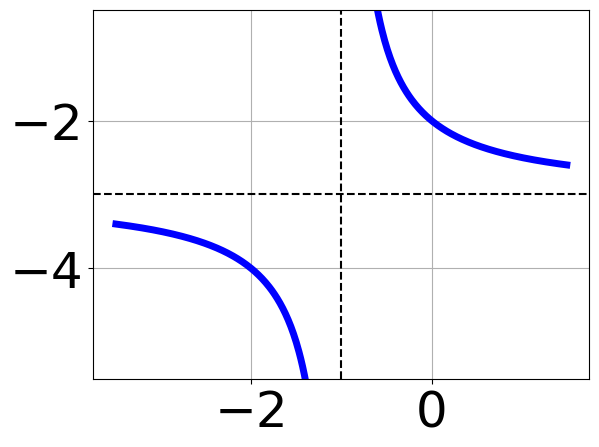
\includegraphics[width = 0.3\textwidth]{../Figures/rationalEquationToGraphAB.png}\item 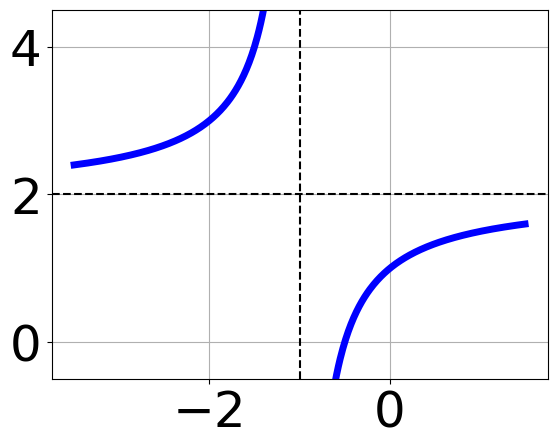
\includegraphics[width = 0.3\textwidth]{../Figures/rationalEquationToGraphBB.png}\item 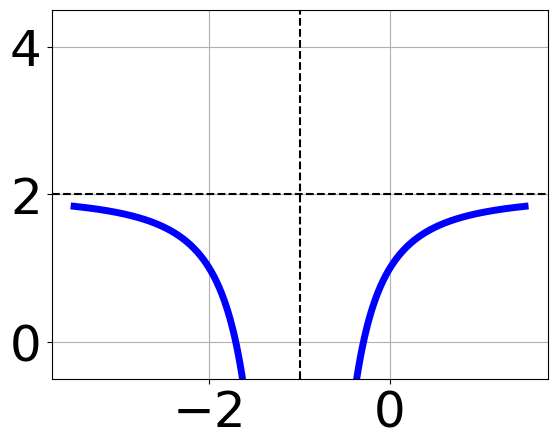
\includegraphics[width = 0.3\textwidth]{../Figures/rationalEquationToGraphCB.png}\item 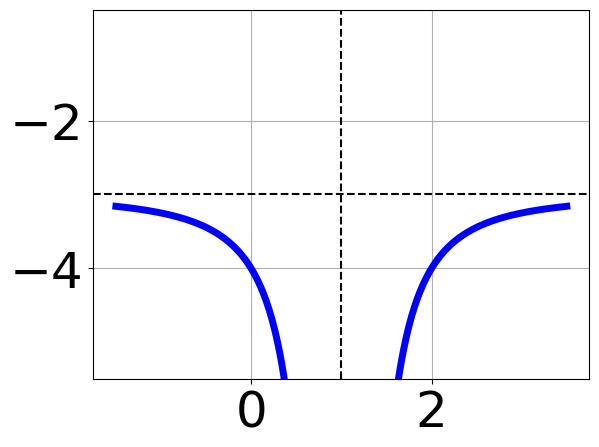
\includegraphics[width = 0.3\textwidth]{../Figures/rationalEquationToGraphDB.png}\end{multicols}\item None of the above.
\end{enumerate} }
\litem{
Choose the graph of the equation below.\[ f(x) = \frac{-1}{x + 1} - 3 \]\begin{enumerate}[label=\Alph*.]
\begin{multicols}{2}\item 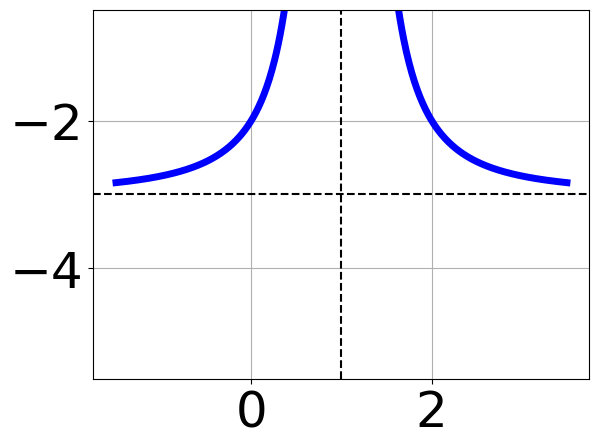
\includegraphics[width = 0.3\textwidth]{../Figures/rationalEquationToGraphCopyAB.png}\item 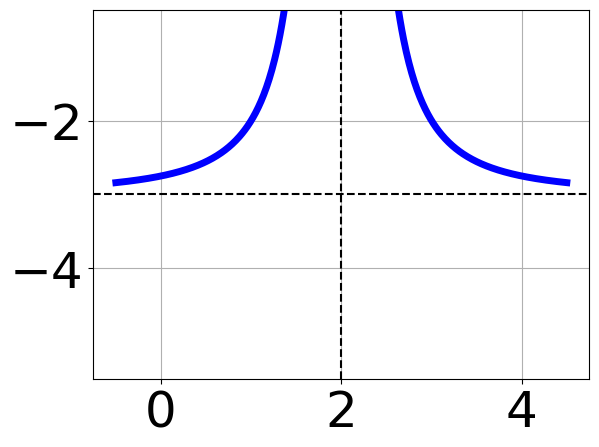
\includegraphics[width = 0.3\textwidth]{../Figures/rationalEquationToGraphCopyBB.png}\item 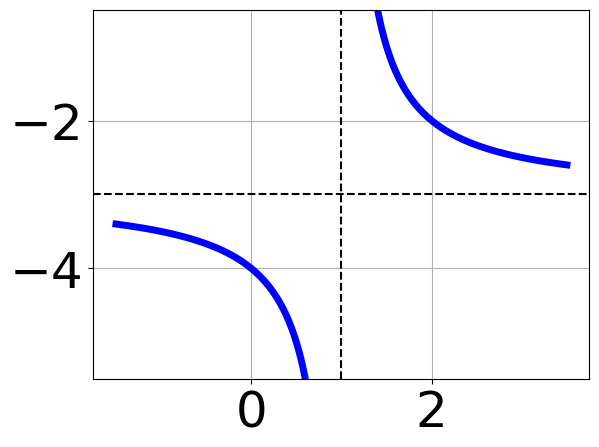
\includegraphics[width = 0.3\textwidth]{../Figures/rationalEquationToGraphCopyCB.png}\item 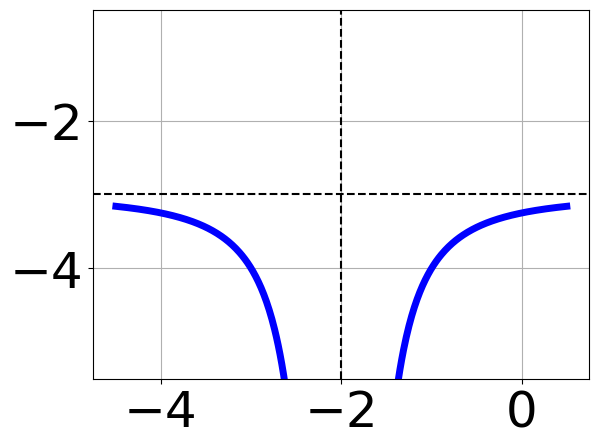
\includegraphics[width = 0.3\textwidth]{../Figures/rationalEquationToGraphCopyDB.png}\end{multicols}\item None of the above.
\end{enumerate} }
\litem{
Choose the equation of the function graphed below.
\begin{center}
    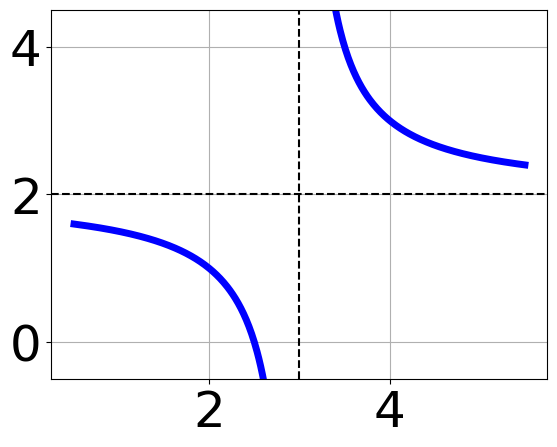
\includegraphics[width=0.5\textwidth]{../Figures/rationalGraphToEquationCopyB.png}
\end{center}
\begin{enumerate}[label=\Alph*.]
\item \( f(x) = \frac{-1}{x - 2} - 3 \)
\item \( f(x) = \frac{1}{(x + 2)^2} - 3 \)
\item \( f(x) = \frac{-1}{(x - 2)^2} - 3 \)
\item \( f(x) = \frac{1}{x + 2} - 3 \)
\item \( \text{None of the above} \)

\end{enumerate} }
\litem{
Solve the rational equation below. Then, choose the interval(s) that the solution(s) belongs to.\[ \frac{-8}{8x -9} + 3 = \frac{-3}{-56x + 63} \]\begin{enumerate}[label=\Alph*.]
\item \( x \in [1.48,3.48] \)
\item \( x \in [-0.91,-0.75] \)
\item \( \text{All solutions lead to invalid or complex values in the equation.} \)
\item \( x_1 \in [1.23, 1.44] \text{ and } x_2 \in [0.48,3.48] \)
\item \( x_1 \in [-0.91, -0.75] \text{ and } x_2 \in [0.48,3.48] \)

\end{enumerate} }
\litem{
Solve the rational equation below. Then, choose the interval(s) that the solution(s) belongs to.\[ \frac{25}{10x -25} + 1 = \frac{25}{10x -25} \]\begin{enumerate}[label=\Alph*.]
\item \( x \in [-3.5,-1.5] \)
\item \( x_1 \in [2.5, 4.5] \text{ and } x_2 \in [2.5,4.5] \)
\item \( \text{All solutions lead to invalid or complex values in the equation.} \)
\item \( x \in [2.5,3.5] \)
\item \( x_1 \in [-3.5, -1.5] \text{ and } x_2 \in [2.5,4.5] \)

\end{enumerate} }
\litem{
Solve the rational equation below. Then, choose the interval(s) that the solution(s) belongs to.\[ \frac{-6x}{4x -7} + \frac{-3x^{2}}{-20x^{2} +55 x -35} = \frac{-4}{-5x + 5} \]\begin{enumerate}[label=\Alph*.]
\item \( x \in [1.16,1.72] \)
\item \( x_1 \in [-1.22, -0.45] \text{ and } x_2 \in [0.67,1.33] \)
\item \( \text{All solutions lead to invalid or complex values in the equation.} \)
\item \( x \in [0.69,1.02] \)
\item \( x_1 \in [-1.22, -0.45] \text{ and } x_2 \in [1.37,2.08] \)

\end{enumerate} }
\litem{
Choose the equation of the function graphed below.
\begin{center}
    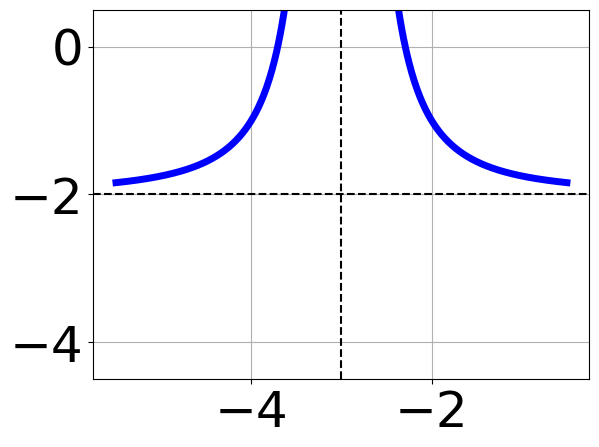
\includegraphics[width=0.5\textwidth]{../Figures/rationalGraphToEquationB.png}
\end{center}
\begin{enumerate}[label=\Alph*.]
\item \( f(x) = \frac{1}{x + 3} - 2 \)
\item \( f(x) = \frac{-1}{x - 3} - 2 \)
\item \( f(x) = \frac{1}{(x + 3)^2} - 2 \)
\item \( f(x) = \frac{-1}{(x - 3)^2} - 2 \)
\item \( \text{None of the above} \)

\end{enumerate} }
\end{enumerate}

\end{document}